
When nonlinear situation is encountered in solving the heat conduction equation, the problem of this kind is handled by means of iteration. It means that the problem is linearised and the solver tries to guess the temperature resolution throughout the domain until the change of temperature between the steps will converge to a desirably low value. Therefore, it is usually computationally costly to solve the quench propagation because one should cope with a temperature distribution being steep at the level of the quench front. Due to high material non-linearities at cryogenic temperatures, in order to accurately solve the temperature distribution in the entire region of the cable, one should refine mesh and/or decrease the simulation time step (up to the order of a $\mu$s).

\begin{figure}[H]
\centering
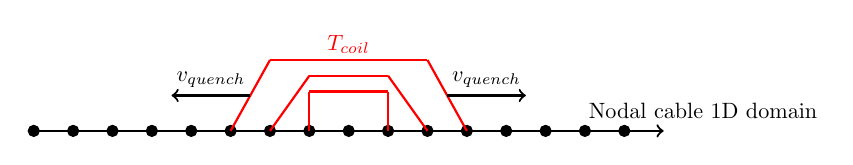
\begin{tikzpicture}[scale = 1]
\draw [thick, ->] (0.0,0.0) -- (8.0,0);
\foreach \t in {0,0.5,1,...,7.5}
\filldraw[black] ({\t},0) circle (2pt);
\node[scale = 0.8] at (8.5,0.25) {Nodal cable 1D domain};
\draw [thick, red] (3.5,0) -- (3.5,0.5);
\draw [thick, red] (3.5,0.5) -- (4.5,0.5);
\draw [thick, red] (4.5,0.5) -- (4.5,0);
\draw [thick, red] (3,0) -- (3.5,0.7);
\draw [thick, red] (3.5,0.7) -- (4.5,0.7);
\draw [thick, red] (4.5,0.7) -- (5,0);
\draw [thick, red] (2.5,0) -- (3,0.9);
\draw [thick, red] (3,0.9) -- (5,0.9);
\draw [thick, red] (5,0.9) -- (5.5,0);
\draw [thick, ->] (5.25,0.45) -- (6.25,0.45);
\node[scale = 0.8] at (5.75,0.65) {$v_\text{quench}$};
\draw [thick, ->] (2.75,0.45) -- (1.75,0.45);
\node[scale = 0.8] at (2.25,0.65) {$v_\text{quench}$};
\node[scale = 0.8, red] at (4,1.1) {$T_\text{coil}$};
\end{tikzpicture}
\caption{Schematic temperature propagation with quench velocity modelling.}
\label{fig:modelling_approach}
\end{figure}

Fig. \ref{fig:modelling_approach} presents an approximated temperature distribution over a discretised 1D thermal domain. The quenched and non-quenched regions in a superconducting cable have different but relatively uniform temperature distributions except for the regions close to the quench front. Therefore, iterating over the regions outside of the quench front to find nodal temperatures is faster and requires less computing power.

The idea of quench velocity modelling bases on predicting quench velocity by an outsourced external routine. Such an approach allows one to have the quench wave explicitly solved. An accurate solution at the quench front is not required and the temperature in this region is approximated, knowing that it is placed between two extreme temperatures (inside or outside of the quenched zone). As a result, the mesh refinement along the coil length is not needed anymore and the numerical model is of a smaller size to be solved. Therefore, the numerical model still calculates the heat balance equation but with a fixed and relatively coarse mesh along the coil of a magnet. 

Solving quench propagation by means of quench velocity method assumes that, while  simulating the heat propagation during quench, the quench front velocity is known and estimated separately beforehand. The quench velocity can be:
\begin{itemize}
\item based on available measurements,
\item calculated analytically based on available formulae,
\item calculated numerically based on short numerical model with refined mesh to solve the quench front with sufficient precision.
\end{itemize}